\documentclass[11pt]{article}

\usepackage[utf8]{inputenc}
\usepackage[T1]{fontenc}
\usepackage{lmodern}
\usepackage{microtype}
\usepackage{amsmath,amssymb,booktabs,tabularx,array,multirow}
\usepackage[margin=1in]{geometry}
\usepackage{graphicx}
\usepackage{caption}
\usepackage{subcaption}
\usepackage{enumitem}
\usepackage[numbers,sort&compress]{natbib}
\usepackage[hidelinks]{hyperref}
\usepackage{xurl}
\usepackage{float}
\setlength{\parskip}{0.35em}
\setlength{\parindent}{1em}
\emergencystretch=2em
\captionsetup{font=small,labelfont=bf}
\renewcommand{\abstractname}{Abstract}
\renewcommand{\tablename}{Table}
\renewcommand{\figurename}{Figure}
\renewcommand{\refname}{References}
\newcommand{\comp}{\textsc{comp}}
\newcommand{\coop}{\textsc{coop}}
\newcommand{\equalself}{\texttt{equal\_self}}
\newcommand{\scarce}{\texttt{scarce}}
\newcommand{\abundant}{\texttt{abundant}}
\newcommand{\logit}{\operatorname{logit}}

\title{The Effect of Resource Scarcity on Competitive Choices by Open-Weight Language Models}
\author{Jacek Rozwadowski\\[2pt]\normalsize Independent Researcher, EdgeNodeLab}
\date{November 2026}

\begin{document}
\maketitle

\begin{abstract}
We examine whether the way a decision-making situation is presented in a prompt changes the choices of open-weight language models when the payoff structure remains unchanged. The task is a one-shot forced A/B choice between a competitive and a cooperative action; we measure the relative next-token logit, averaged over both option orders. We tested 12 model variants (Base and Instruct versions of Qwen2.5 in three sizes, Mistral-7B, Bielik-11B-v3, and Gemma-4-12B), two languages (English and Polish), three actor labels, three action descriptions, five payoff structures, and two resource-availability contexts (41\,472 evaluations). Inference is based on paraphrase templates rather than individual prompts. Seven variants passed the measurement-validity checks (probability mass on A/B and accuracy on dominance controls); the remaining five were excluded from the main analysis, and their results are reported in a sensitivity analysis.

In the main equal-own-payoff condition (\equalself), the resource-scarcity sentence increases the competitive-choice logit in all seven retained variants (from 0.15 to 1.93 logits; on the probability scale, from 2.3 to 12.9 percentage points); in six of them, the effect meets the Bonferroni threshold (0.0018), while for Qwen2.5-14B-Instruct it is nominally significant but does not meet the threshold. The effect is also positive in the other five excluded variants. For Qwen2.5-3B and 7B, the effect is substantially larger in the Instruct variants than in the Base variants, but these variants used different prompting protocols, and the effect is small in Qwen2.5-14B-Instruct, so the difference cannot be attributed to instruction tuning. The direction of the effect of charged action descriptions (\texttt{charged} vs.\ \texttt{plain}) and the effects of actor labels are not consistent across models. An exploratory analysis of the dominance controls indicates that the descriptions “independently”/“jointly” shift choices toward the cooperative option in six of the seven variants, whereas neutral X/Y labels do not.

The results concern conditional next-token distributions in artificial prompts, not the models' goals or persistent preferences. The model inclusion criterion was changed after earlier results had been observed, models were added in successive runs, and inference is based on six paraphrases per language; the conclusions are therefore considered preliminary.
\end{abstract}

\noindent\textbf{Keywords:} large language models; social decisions; cooperation; competition; resource-scarcity framing;
prompt sensitivity; logit-based evaluation; bilingual evaluation

\section{Introduction}
Large language models (LLMs) are increasingly used in processes where their recommendations can affect the interests of multiple stakeholders. Their behavior in strategic decision-making settings with social consequences is therefore an issue that requires empirical investigation, rather than something that can be inferred solely from the fluency of generated language. Recent studies have examined LLM behavior in repeated games, one-shot social dilemmas, and tasks requiring coordination. These studies point both to models' ability to adapt their strategies usefully and to substantial sensitivity of their behavior to task structure and how the situation is presented \citep{phelps2025machine,akata2025repeated,tewolde2026coopeval,pal2026robust}.

One recurring methodological problem is the difficulty of separating a genuine preference for cooperation from other factors, such as a model's ability to read payoff tables correctly, the semantic valence of action descriptions, or a tendency to choose the first or second option. A model that chooses an action described as cooperative may be responding primarily to the wording used rather than to the payoff structure. Conversely, a model that fails a payoff-dominance test may appear prosocial simply because it compares numerical values incorrectly.

In this study, we use a paired forced-choice design that makes it possible to disentangle the effects of several of these factors. The main outcome variable is the relative probability assigned to competitive and cooperative options, estimated from the next-token logits corresponding to the response labels. Each scenario is presented twice, with the option order reversed. We also use two control payoff structures based on dominance to test whether a model can choose the option that is beneficial to both parties, regardless of whether its description suggests competition or cooperation. The main study condition, designated \equalself, keeps the decision-maker's payoff at the same level for both possible actions, while making competition worsen the outcome for the other party.

The study focuses on three hypotheses and one exploratory question:

\begin{enumerate}[leftmargin=2.4em,itemsep=0.15em,label=\textbf{H\arabic*:}]
    \item A charged action description (\texttt{charged}), compared with a \texttt{plain} description, reduces the probability of choosing competition in the \equalself{} condition (a hypothesis derived from earlier observations; see Section~\ref{sec:stats}).
    \item The actor label (tribe, team, agent) systematically affects competitive choices.
    \item Information about resource scarcity increases the probability of choosing competition when the stated payoffs remain unchanged (a hypothesis also derived from earlier observations).
    \item[\textbf{Q:}] How large are choice shifts resulting from wording compared with the effect of unequivocally dominant numerical payoffs? (exploratory analysis)
\end{enumerate}

The most consistent finding is the positive effect of presenting the situation as one of resource scarcity, observed in all seven model variants that passed the adopted diagnostic procedures (and surviving Bonferroni correction in six of them). Effects associated with action descriptions and actor labels are considerably less consistent. We emphasize that the experiment measures prompt-conditioned model responses in an artificially constructed one-shot resource-allocation scenario. It does not provide evidence that models possess internal preferences, intentions, or autonomous social goals.

\section{Related Work}
\paragraph{Prompt wording and social preferences.}
Phelps and Russell investigate whether descriptions expressing cooperative, competitive, altruistic, and self-interested orientations can change the behavior of GPT-3.5 in a repeated prisoner's dilemma and a dictator game. The authors suggest that natural-language character descriptions can translate into corresponding behavior in the tasks, particularly in one-shot situations \citep{phelps2025machine}. The linguistic manipulation used in our study is narrower in scope: it changes the descriptions of the two available actions while keeping their payoffs unchanged. It also includes neutral action labels as a reference condition.

\paragraph{Language models in strategic games.}
Akata and colleagues use methods from behavioral game theory to evaluate language models in finitely repeated two-player games. They identify differences between games based on self-interest and tasks requiring coordination, as well as model sensitivity to additional social information \citep{akata2025repeated}. Pal and colleagues analyze strategies in the repeated prisoner's dilemma, payoff variation, and alternative ways of presenting the situation. Their results indicate that contemporary models can exhibit consistent cooperative strategies under certain conditions, but do not remain fully consistent across all tested variants \citep{pal2026robust}. These studies concern repeated interactions and strategy adaptation across successive rounds, whereas the present experiment focuses on a single choice with predetermined payoffs for both parties.

Tewolde and colleagues introduce CoopEval, a benchmark comprising several types of social dilemmas and mechanisms that support the maintenance of cooperation. In their experiments, they observed a substantial proportion of defection in one-shot mixed-motive games among the models they tested. They also showed that institutional mechanisms can affect cooperation-related outcomes \citep{tewolde2026coopeval}. The task used in our study is neither a prisoner's dilemma nor a repeated strategic game. It consists of a unilateral choice between two possible outcomes, specified from the perspective of the decision-maker and the other party. This simpler structure makes it possible to manipulate the decision-maker's payoff, the other party's payoff, and the context and wording of the situation description directly.

\paragraph{Positioning and contribution of the present study.}
The aim of this paper is to make a primarily methodological and diagnostic contribution, rather than to produce a general ranking of language models according to their propensity for prosocial behavior. The research design combines five elements: (i) reversing the order in which options are presented, (ii) control scenarios with dominant payoff structures, (iii) a condition with equal payoffs for the decision-maker, (iv) semantically neutral and charged action descriptions, and (v) paraphrase templates in English and Polish. The results make it possible to assess whether the effect of how a situation is presented persists when the model demonstrates an ability to correctly identify numerical dominance under the condition using neutral action labels.

\section{Experimental Design}
\subsection{Task and payoff structures}
Each prompt describes a situation in which two parties draw on a shared pool of resources. The decision-maker must choose between a competitive action and a cooperative action. The outcome of each action is represented as an ordered pair of values, \((u_{\mathrm{self}},u_{\mathrm{other}})\), where the first value denotes the payoff of the party making the decision and the second denotes the payoff of the other party.

The task is a one-shot decision scenario in which one party makes a choice based on specified payoffs. It does not model two players making simultaneous strategic decisions.

Five payoff structures were used in the experiment. Three constitute the core experimental conditions, while two serve as dominance controls. The core experimental conditions were evaluated using two payoff scales (multipliers of 1 and 2), whereas only one scale was used for the control conditions.

\begin{table}[H]
\centering
\small
\caption{Payoff structures. Each ordered pair represents (decision-maker's payoff, other party's payoff).}
\begin{tabular}{lccp{5.6cm}}
\toprule
Condition & Competitive action & Cooperative action & Interpretation \\
\midrule
\texttt{comp\_dominant} & $(8,3)$ & $(5,5)$ & Competition increases the decision-maker's payoff while simultaneously reducing the other party's payoff. \\
\texttt{coop\_dominant} & $(5,3)$ & $(8,8)$ & Compared with competition, cooperation benefits both parties. \\
\texttt{equal\_self} & $(6,2)$ & $(6,6)$ & The decision-maker's payoff is identical for both actions; competition reduces the other party's payoff. \\
\texttt{dom\_comp} & $(8,8)$ & $(4,3)$ & The competitive action is strictly better for both parties (dominance control). \\
\texttt{dom\_coop} & $(4,3)$ & $(8,8)$ & The cooperative action is strictly better for both parties (dominance control). \\
\bottomrule
\end{tabular}
\label{tab:payoffs}
\end{table}


The \equalself{} condition is the main condition for outcome analysis. Since both actions provide the decision-maker with a payoff of 6 units, a preference for the competitive action cannot be explained by a higher stated personal payoff. Such a choice may, however, result from how the prompt is interpreted, semantic associations, a response bias (e.g., toward a particular label or position), or other unobserved mechanisms of model behavior. The task design does not make it possible to determine which of these causes accounts for the choice made.

\subsection{Experimental factors}
The prompt generator combines the following experimental factors:

\begin{itemize}[leftmargin=1.5em,itemsep=0.1em]
\item \textbf{Language:} English and Polish.
\item \textbf{Actor label:} agents (Agent A and Agent B), teams (the decision-maker's team and the other team), or tribes (the decision-maker's tribe and the rival tribe).
\item \textbf{Action description:} \texttt{charged}, \texttt{plain}, or \texttt{label}.
\item \textbf{Payoff structure:} the five conditions presented in Table~\ref{tab:payoffs}.
\item \textbf{Situational context:} a sentence indicating resource scarcity (there are not enough resources for everyone) or abundance (there are more resources than everyone needs).
\item \textbf{Template:} six paraphrases for each language.
\item \textbf{Option order:} the competitive option first or the cooperative option first.
\end{itemize}

The three action-description variants deliberately differ in semantic content. In the English prompts, the \texttt{charged} variant contrasts the phrases “Seize control of the pool and push the other side out” and “Join forces with the other side and manage the pool together.” The \texttt{plain} variant contrasts “Act on the pool independently” and “Act on the pool jointly with the other side.” The \texttt{label} variant uses the terms “Action X” and “Action Y,” whose assignment to competitive and cooperative payoffs is alternated across generated scenarios. Corresponding translations were used in the Polish prompts (e.g., “Działać na puli samodzielnie,” “Działanie X”). The translations were not checked by a second native speaker (see Section~\ref{sec:limits}).

The \texttt{plain} variant is not semantically neutral: it explicitly indicates acting independently or jointly. Nor does the \texttt{charged} variant constitute a clean manipulation of emotional intensity. It combines several elements: evaluative valence, the way agency is represented, and the description of the action itself.

The actor label is also associated with different resource names: for tribes, these are food rations; for teams, budget units; and for agents, resource units. In addition, the labels “Agent A” and “Agent B” coincide with the response letters A and B, which may have affected how the prompt was read. Accordingly, differences between actor variants should be interpreted as a comparison of entire ways of representing participants and types of resources, rather than as an isolated measure of the effect of social identity.

The resource-scarcity manipulation consists solely of changing the sentence that introduces the scenario. It does not change the payoff matrix, the size of the available pool, or the feasibility of either action. We therefore speak of a textual framing of the situation as one of scarcity, not of a manipulation of actual material scarcity.

\subsection{Number of prompts and pairing procedure}
The generator creates 3456 prompts for each model variant, corresponding to 1728 scenario pairs. Each pair contains identical content and payoff structure but differs in the order in which the competitive and cooperative options are presented. Six templates were used for each language. Two value scales were used for the main payoff structures, whereas one scale was used for the dominance controls. In total, 41\,472 prompts were evaluated across the twelve model variants.

\subsection{Models and inference configuration}\label{sec:models}
Twelve language-model variants were evaluated in the experiment (six families in Base and Instruct versions):

\begin{itemize}[leftmargin=1.5em,itemsep=0.1em]
\item \textbf{Qwen2.5-3B:} \url{Qwen/Qwen2.5-3B}, \url{Qwen/Qwen2.5-3B-Instruct}
\item \textbf{Qwen2.5-7B:} \url{Qwen/Qwen2.5-7B}, \url{Qwen/Qwen2.5-7B-Instruct}
\item \textbf{Qwen2.5-14B:} \url{Qwen/Qwen2.5-14B}, \url{Qwen/Qwen2.5-14B-Instruct}
\item \textbf{Mistral-7B:} \url{mistralai/Mistral-7B-v0.1}, \url{mistralai/Mistral-7B-Instruct-v0.2}
\item \textbf{Bielik-11B-v3} (Polish open model): \url{speakleash/Bielik-11B-v3-Base-20250730}, \url{speakleash/Bielik-11B-v3.0-Instruct}
\item \textbf{Gemma-4-12B:} \url{google/gemma-4-12B}, \url{google/gemma-4-12B-it}
\end{itemize}

Qwen2.5-3B and Gemma-4-12B were loaded at FP16 precision, while Qwen2.5-7B, Qwen2.5-14B, Mistral-7B, and Bielik-11B used 4-bit quantization. The experiment was configured to run in an environment equipped with a CUDA-capable graphics processor.

The base models (Base) received a few-shot prefix containing eight examples. The examples used neutral action descriptions (“Move 1” / “Move 2”), a balanced distribution of response labels (four A responses and four B responses), and scenarios covering both conflicts of interest and situations without conflict. In six of the eight examples, the two options have different own payoffs, and the indicated response is always the option with the higher own payoff; in the remaining two, own payoffs are equal (in one, the indicated option has a lower payoff for the other party, and in the other, a higher one). The examples therefore primarily teach maximization of one's own payoff, which may affect choices in the \equalself{} condition and in the dominance controls. Scarcity and abundance contexts alternate across the examples.

The instruction-tuned models (Instruct) received prompts prepared using the appropriate conversational template (chat template), containing an instruction to respond with exactly one letter. They did not receive a few-shot prefix.

In addition, Mistral-Instruct and Gemma-Instruct used an assistant-response prefill with the text “Answer:” (Mistral) or “Reply:” (Gemma) in English prompts, and “Odpowiedź:” in Polish prompts (a duplicated BOS token was removed in this process); in the Gemma chat template, the end of the prompt also contained an empty reasoning block (\texttt{<|channel>thought}).

This means that comparing Base and Instruct variants is not a controlled intervention involving only a change in model weights. The model variant, conversation formatting, presence of few-shot context, and preparation of the final part of the prompt all change simultaneously. Consequently, the observed differences between Base and Instruct variants cannot be attributed solely to instruction tuning.

\section{Response Evaluation and Statistical Analysis}
\subsection{Paired measurement of next-token probability}
For each prompt, the measurement procedure identifies single-token variants of the response labels A and B, also accounting for variants preceded by a space. Let $V_A$ and $V_B$ denote the sets of token IDs corresponding to these labels. The sets include, among others, the forms “A”, “ A”, “\textunderscore A”, and “ĠA” (and analogously for B). The next-token probabilities assigned to individual variants are summed within each set (the calculation was performed on the logarithmic scale using logsumexp):

\begin{equation}
    q_A = \sum_{t\in V_A} P(t\mid x),\qquad
    q_B = \sum_{t\in V_B} P(t\mid x).
\end{equation}

The conditional probability of response A, assuming that the response will be expressed using one of the two permitted labels, is calculated as follows:

\begin{equation}
    p_A = \frac{q_A}{q_A+q_B}.
\end{equation}

If the competitive option is designated by the letter A, then $p_{\mathrm{comp}}=p_A$; otherwise, $p_{\mathrm{comp}}=1-p_A$. Before calculating the logit, $p_{\mathrm{comp}}$ is clipped to the interval $[10^{-4},\,1-10^{-4}]$, which limits the absolute value of the logit to approximately 9.21. The corresponding competitive-choice logit is:

\begin{equation}
    z=\logit(p_{\mathrm{comp}})=\log\left(\frac{p_{\mathrm{comp}}}{1-p_{\mathrm{comp}}}\right).
\end{equation}

For each scenario, both presentations that differ in option order are converted to the logit of choosing competition and then averaged. This operation eliminates a constant additive model preference for response A over B, assuming that the position effect is approximately symmetric in the two presentations with reversed option order. However, it does not guarantee the elimination of interactions between response position and prompt wording or payoff structure.

We additionally monitor the quantity referred to as \texttt{mass} (the probability mass assigned to the labels):
\begin{equation}
    \texttt{mass}=q_A+q_B.
\end{equation}

A value close to one means that the model assigns most of its next-token probability to one of the two permitted response labels. The mean value of this measure is reported for each model in Table~\ref{tab:diagnostics}. Because the choice outcome is normalized only with respect to responses A and B, all reported choice probabilities are conditional on these two labels.

\subsection{Aggregation of results and uncertainty estimation}\label{sec:stats}
In the first stage of the analysis, the results obtained for the two presentations of the same scenario, which differ in reversed option order, are averaged. Next, for the main experimental conditions, the results obtained for the two payoff scales within each cell of the research design are averaged.

For statistical inference, one effect is computed per paraphrase template, separately for each language (six per language). The reported point estimate is the arithmetic mean of two means: the one obtained for English and the one obtained for Polish, with equal weight assigned to both languages. A confidence interval based on Welch's $t$ distribution is used, with six template-level observations for each language. Differences between languages (Polish minus English) are reported separately and exploratorily, without correction for multiple comparisons (Section~\ref{sec:lang}).

The unit of statistical inference is therefore the paraphrase template, not an individual prompt. The reported confidence intervals reflect variation in results across the six templates used for each language, applying the statistical procedure described above. They are not confidence intervals derived from sampling individual prompts and do not provide a basis for generalizing the results to arbitrary prompts not used in the experiment or to other model checkpoints.

Four primary contrasts are analyzed in the main \equalself{} condition:

\begin{enumerate}[leftmargin=1.6em,itemsep=0.15em]
\item \texttt{charged} minus \texttt{plain};
\item \texttt{tribe} minus \texttt{agent};
\item \texttt{team} minus \texttt{agent};
\item resource scarcity (\texttt{scarce}) minus resource abundance (\texttt{abundant}).
\end{enumerate}

Seven model variants meet the adopted diagnostic criteria, leading to a Bonferroni-corrected statistical significance threshold of $0.05/(4\times7)\approx0.0018$ for tests of individual contrasts in each model. Results for the remaining five variants are presented outside the main analysis, in Appendix~\ref{app:sens}.

The hypotheses concerning action descriptions and the resource-scarcity context were formulated based on earlier experimental observations. Accordingly, the present study is a replication of those observations using new paraphrases (the same prompt family and the same measurement pipeline), rather than a study based entirely on a preregistered analysis plan. In addition, the criteria for assessing measurement validity and model inclusion were changed after the initial analysis of the results. These circumstances limit the strength of statistical inference; therefore, the results should be interpreted with caution, and the conclusions drawn from them should be regarded as preliminary and requiring further verification.

\subsection{Decomposition of dominance-control results}
In the two dominance-control conditions, the payoff structure unambiguously indicates which action is more advantageous. Let $m_{\comp}$ denote the logit margin in favor of choosing the competitive action in the \texttt{dom\_comp} condition, and let $m_{\coop}$ denote the corresponding margin in favor of choosing the cooperative action in the \texttt{dom\_coop} condition. The following quantities are calculated for each model and each action-description variant (\texttt{numbers} -- sensitivity to numerical advantage; \texttt{lean} -- shift toward the option described as cooperative):

\begin{equation}
\text{numbers}=\frac{m_{\coop}+m_{\comp}}{2},\qquad
\text{lean}=\frac{m_{\coop}-m_{\comp}}{2}.
\end{equation}

Under the assumption of additivity on the logit scale, the \texttt{numbers} variable measures the model's sensitivity to the direction of dominance resulting from the payoff structure, whereas \texttt{lean} measures a systematic shift toward the option described using cooperative language, regardless of which option is numerically more advantageous.

This decomposition is exploratory and is based on the assumption that effects are additive on the logit scale. A value of \texttt{lean} close to zero in the condition using neutral action labels provides a useful internal check of the validity of the adopted measurement method. By itself, however, it does not confirm that this quantity is a valid measure of a psychological construct.

\section{Measurement Validity Diagnostics}
According to the adopted analytical procedure, a model was included in further analyses only if it simultaneously met two criteria:

\begin{enumerate}
\item The mean probability mass assigned jointly to responses A and B exceeded $90\%$.
\item The sign of the paired logit indicated selection of the payoff-dominant option in at least $90\%$ of the pairs of control scenarios with neutral action labels, considering all actor labels jointly.
\end{enumerate}

The second criterion was changed after reviewing the earlier experimental results and is therefore post hoc, meaning that it was specified after the data had been initially analyzed.

\begin{table}[H]
\centering
\small
\caption{Measurement-validity diagnostics for all twelve variants. ``Label control'' denotes the proportion of correct selections, determined from the sign of the logit, in dominance-control scenarios using neutral action labels. ``All wording'' denotes the combined results for all action-description variants used.}

\begin{tabular}{lccccc}
\toprule
Model variant & A/B mass & Label control & All wording & $P(A)$ mean & Retained \\
\midrule
Bielik-11B-v3 base      & 0.973 & 1.000 & 0.975 & 0.596 & Yes \\
Bielik-11B-v3 instruct  & 0.886 & 0.799 & 0.868 & 0.314 & No \\
Gemma-4-12B base        & 0.988 & 0.681 & 0.773 & 0.703 & No \\
Gemma-4-12B instruct    & 0.946 & 0.292 & 0.417 & 0.606 & No \\
Mistral-7B base         & 0.957 & 0.993 & 0.958 & 0.451 & Yes \\
Mistral-7B instruct     & 0.967 & 0.556 & 0.576 & 0.961 & No \\
Qwen2.5-3B base         & 0.938 & 0.986 & 0.762 & 0.441 & Yes \\
Qwen2.5-3B instruct     & 1.000 & 0.931 & 0.944 & 0.366 & Yes \\
Qwen2.5-7B base         & 0.953 & 1.000 & 0.887 & 0.322 & Yes \\
Qwen2.5-7B instruct     & 1.000 & 0.924 & 0.845 & 0.490 & Yes \\
Qwen2.5-14B base        & 0.966 & 0.889 & 0.928 & 0.631 & No \\
Qwen2.5-14B instruct    & 0.980 & 0.972 & 0.773 & 0.437 & Yes \\
\bottomrule
\end{tabular}
\label{tab:diagnostics}
\end{table}

The criteria were not changed relative to version v3.2; the Bielik-11B-v3 and Gemma-4-12B models were added after they had been established. Five variants do not meet the criteria: Mistral-7B-Instruct (neutral-label control accuracy 0.556, and also a strong first-option preference, $P(A)=0.961$), Bielik-11B-v3-Instruct (A/B mass 0.886, accuracy 0.799), Gemma-4-12B-Base (accuracy 0.681), Gemma-4-12B-Instruct (accuracy 0.292, i.e. below chance level; a batched-versus-single-example evaluation check revealed large discrepancies for this variant (see Limitations), so the result is most likely a measurement artifact rather than model behavior), and Qwen2.5-14B-Base, which narrowly misses the threshold (accuracy 0.889 against the required 0.9). Estimates for these variants are not interpreted substantively in the main analysis; their results are compiled in Appendix~\ref{app:sens}.

Among the variants that passed diagnostics, Qwen2.5-7B-Instruct has lower neutral-label control accuracy for the agent actor (0.83) than for the team (0.96) and tribe (0.98); comparisons involving individual actor types for this model should be interpreted with particular caution.

In several models, control accuracy calculated jointly across all action-description variants is lower than the accuracy obtained using neutral labels alone; this is most pronounced in Qwen2.5-14B-Instruct (0.972 for labels versus 0.773 for all descriptions). In this model, in the \texttt{dom\_comp} control with the \texttt{charged} description, the sign of the logit indicates the correct option in only 10\% of pairs: the model chooses the action description that sounds cooperative even though the other action is better for both parties. This is consistent with the idea that the action description may interfere with choices based on numerical payoff analysis (see, however, the limitation concerning consistency of \texttt{dom\_comp} for the \texttt{charged} description).

\section{Results}
\subsection{Choice of the competitive action by payoff structure}
Table~\ref{tab:payoffmeans} presents descriptive mean probabilities of choosing the competitive action, calculated after averaging the results for scenario presentations with reversed option order. These values are not contrasts used for statistical inference at the template level and should be interpreted solely as descriptive statistics.

\begin{table}[H]
\centering
\small
\caption{Mean probability of choosing the competitive action by payoff structure. Variants that did not pass diagnostics (see Table~\ref{tab:diagnostics}) are included solely to provide a complete overview of the data and are omitted from the interpretation of results.}
\begin{tabular}{lccc}
\toprule
Model variant & \texttt{comp\_dominant} & \texttt{coop\_dominant} & \texttt{equal\_self} \\
\midrule
Bielik-11B-v3 base      & 0.621 & 0.414 & 0.509 \\
Bielik-11B-v3 instruct  & 0.600 & 0.289 & 0.448 \\
Gemma-4-12B base        & 0.739 & 0.323 & 0.488 \\
Gemma-4-12B instruct    & 0.593 & 0.514 & 0.577 \\
Mistral-7B base         & 0.567 & 0.410 & 0.469 \\
Mistral-7B instruct     & 0.485 & 0.455 & 0.485 \\
Qwen2.5-3B base         & 0.477 & 0.377 & 0.380 \\
Qwen2.5-3B instruct     & 0.610 & 0.138 & 0.196 \\
Qwen2.5-7B base         & 0.490 & 0.283 & 0.341 \\
Qwen2.5-7B instruct     & 0.526 & 0.155 & 0.290 \\
Qwen2.5-14B base        & 0.584 & 0.280 & 0.380 \\
Qwen2.5-14B instruct    & 0.222 & 0.041 & 0.090 \\
\bottomrule
\end{tabular}
\label{tab:payoffmeans}
\end{table}

Across all seven model variants included in the analysis, the mean probability of choosing competition is higher in the \texttt{comp\_dominant} condition than in the \texttt{coop\_dominant} condition. The largest difference was observed for Qwen2.5-3B-Instruct (difference of 0.472).
In the \equalself{} condition, the descriptive mean probability of choosing the competitive action is: 0.509 for Bielik-11B-v3-Base, 0.469 for Mistral-7B-Base, 0.380 for Qwen2.5-3B-Base, 0.196 for Qwen2.5-3B-Instruct, 0.341 for Qwen2.5-7B-Base, 0.290 for Qwen2.5-7B-Instruct, and 0.090 for Qwen2.5-14B-Instruct.
These values, however, mask substantial variation depending on the action-description variant and situational context. For Qwen2.5-14B-Instruct, the mean probability is very low (0.090), which means that the logit contrasts for this model are determined close to the lower boundary of the scale, and clipping probabilities at $10^{-4}$ may attenuate them. This issue is examined in the following subsections; Figure~\ref{fig:equalself} shows the descriptive rates.

\begin{figure}[H]
\centering
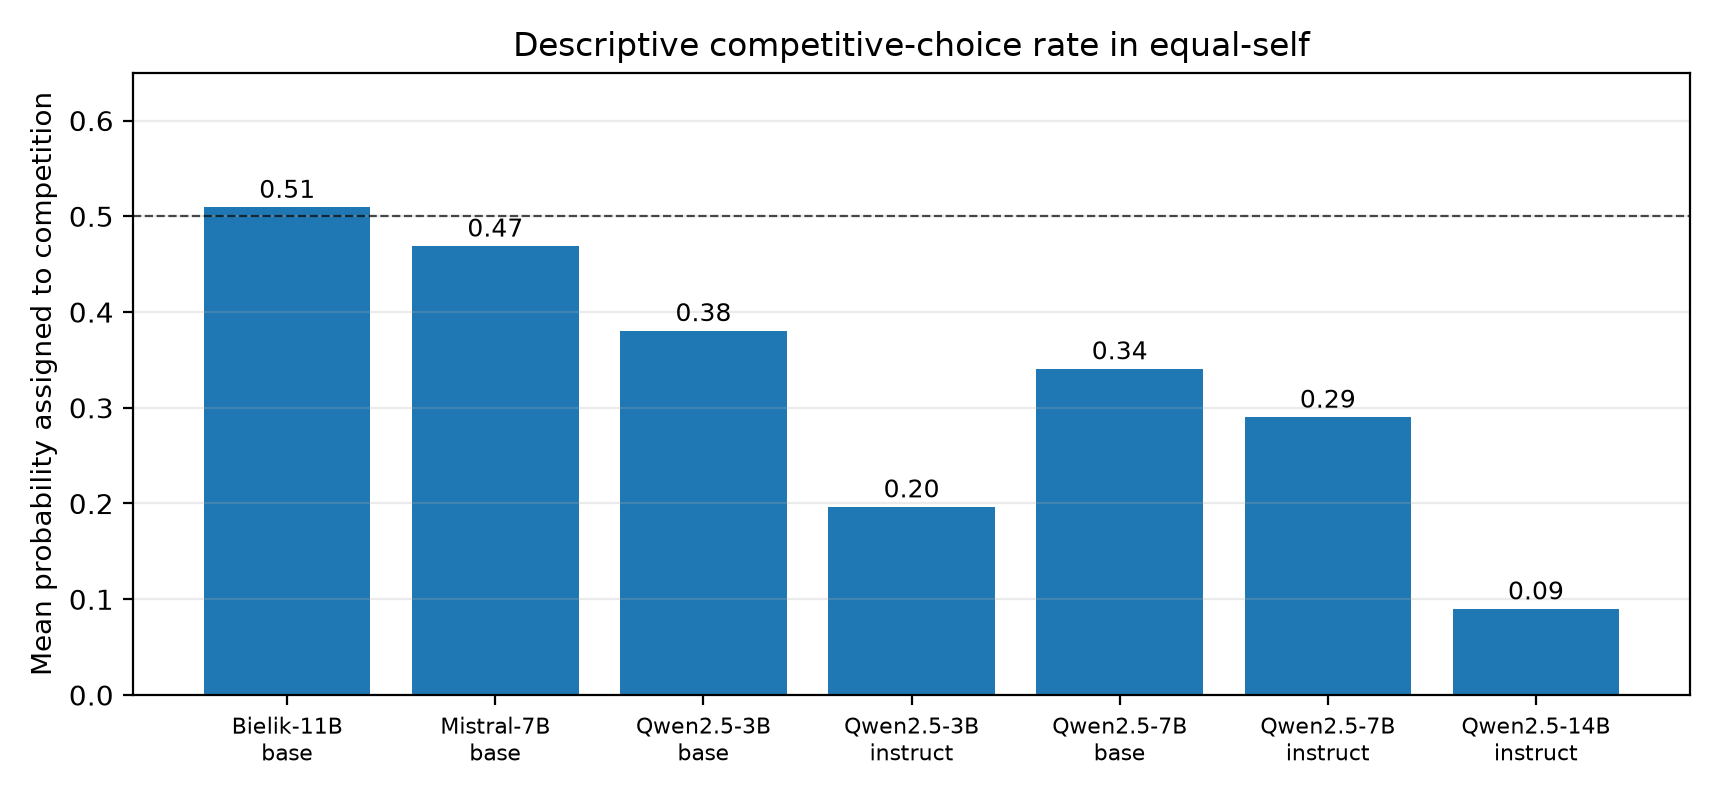
\includegraphics[width=0.82\linewidth]{figs/equal_self_rates.png}
\caption{Descriptive probability of choosing the competitive option in the \equalself{} condition, averaged across all actor variants, action descriptions, languages, situational contexts, payoff scales, and both option orders, for the seven variants that passed diagnostics. The dashed line indicates the 0.5 level.}
\label{fig:equalself}
\end{figure}

\subsection{Main effects in the equal-own-payoff condition}
A positive contrast value indicates a higher competitive-choice logit in the first condition named in the given contrast. Effect estimates and their corresponding 95\% confidence intervals, calculated at the template level, are presented in Table~\ref{tab:primaryeffects}.

\begin{table}[H]
\centering
\scriptsize
\caption{Main logit contrasts in the \equalself{} condition for the seven variants that passed diagnostics. Values are presented as effect estimates with 95\% confidence intervals (template-level $t$ intervals). Positive values indicate a higher logit for choosing the competitive action.}

\begin{tabular}{lcccc}
\toprule
Model variant & Charged $-$ plain & Tribe $-$ agent & Team $-$ agent & Scarce $-$ abundant \\
\midrule
Bielik-11B-v3 base & $-0.05\,[-0.15,0.05]$ & $0.20\,[0.08,0.31]$ & $0.08\,[-0.05,0.21]$ & $0.16\,[0.10,0.23]$ \\
Mistral-7B base & $0.38\,[0.26,0.49]$ & $-0.01\,[-0.09,0.08]$ & $0.01\,[-0.05,0.07]$ & $0.15\,[0.10,0.19]$ \\
Qwen2.5-3B base & $0.02\,[-0.09,0.13]$ & $-0.11\,[-0.24,0.03]$ & $-0.07\,[-0.15,0.01]$ & $0.21\,[0.15,0.27]$ \\
Qwen2.5-3B instruct & $0.09\,[-1.08,1.26]$ & $-0.01\,[-1.74,1.72]$ & $-1.00\,[-2.41,0.40]$ & $1.03\,[0.80,1.26]$ \\
Qwen2.5-7B base & $0.12\,[-0.00,0.24]$ & $0.21\,[0.07,0.35]$ & $0.10\,[-0.05,0.25]$ & $0.22\,[0.15,0.29]$ \\
Qwen2.5-7B instruct & $-2.26\,[-3.66,-0.85]$ & $-0.40\,[-1.97,1.16]$ & $-0.51\,[-1.84,0.82]$ & $1.93\,[1.53,2.34]$ \\
Qwen2.5-14B instruct & $-0.37\,[-1.12,0.39]$ & $1.01\,[0.12,1.89]$ & $1.07\,[0.17,1.97]$ & $0.43\,[0.07,0.79]$ \\
\bottomrule
\end{tabular}
\label{tab:primaryeffects}
\end{table}

\paragraph{H1: charged versus neutral action descriptions (\texttt{charged} vs.\ \texttt{plain}).}
The predicted effect was negative: we expected the charged action description to reduce the probability of choosing competition compared with the neutral description. The observed effect, however, is not consistent across models. Mistral-7B Base exhibits a positive contrast of 0.38 ($p<0.0001$), which is statistically significantly different from zero but in the opposite direction to the stated hypothesis. For Qwen2.5-3B Base, Qwen2.5-3B-Instruct, and Bielik-11B-v3 Base, estimates are close to zero, with confidence intervals including zero. The result for Qwen2.5-7B Base is also close to zero ($p=0.0507$), while that for Qwen2.5-14B-Instruct is negative but has a wide interval ($-0.37$, $p=0.2823$). Qwen2.5-7B-Instruct shows a negative effect estimate ($-2.26$, $p=0.0061$), but it does not meet the Bonferroni-corrected significance threshold of 0.0018. Thus, the experiment does not provide evidence that a charged action description, compared with a neutral one, produces an effect in the predicted direction that is shared across different models.

\paragraph{H2: actor label.}
None of the analyzed actor contrasts shows a stable effect across all included model variants, and none meets the corrected significance threshold. The largest nominal signals were observed for the tribe-minus-agent contrast in Bielik-11B-v3 Base ($0.20$, $p=0.0033$) and Qwen2.5-7B Base ($0.21$, $p=0.0086$); in Qwen2.5-14B-Instruct, both the tribe-minus-agent and team-minus-agent contrasts are positive, but have wide intervals ($p=0.0295$ and $p=0.0243$). The signs of the contrasts vary across models. Given the association of actor labels with different resource names and the lower accuracy of numerical controls for the agent actor in Qwen2.5-7B-Instruct, the data do not provide robust evidence that actor labels alone systematically affect the choice of competition.

\paragraph{H3: resource-scarcity context.}
The resource-scarcity-minus-abundance contrast (\texttt{scarce} minus \texttt{abundant}) is positive in all seven included model variants. In six of them, it meets the main corrected significance threshold; the exception is Qwen2.5-14B-Instruct ($0.43$, $p=0.0233$), where the confidence interval does not include zero, but the p-value exceeds the 0.0018 threshold. The estimated effects range from 0.15 to 1.93 logit units. The corresponding odds ratios are approximately: 1.18 (Bielik-11B-v3-Base), 1.16 (Mistral-7B-Base), 1.23 (Qwen2.5-3B-Base), 2.80 (Qwen2.5-3B-Instruct), 1.25 (Qwen2.5-7B-Base), 6.92 (Qwen2.5-7B-Instruct), and 1.54 (Qwen2.5-14B-Instruct). These ratios describe the change in the odds of choosing the competitive option, conditional on the two permitted response labels. They should not be equated with an absolute change in probability.

\begin{table}[H]
\centering
\small
\caption{Absolute mean probability of choosing competition in the \equalself{} condition under scarcity and abundance (averaged over actors, action descriptions, languages, scales, and both option orders), and the difference in percentage points. Descriptive values, without confidence intervals.}
\begin{tabular}{lccc}
\toprule
Model variant & $P(\mathrm{comp})$ scarce & $P(\mathrm{comp})$ abundant & Difference (pp) \\
\midrule
Bielik-11B-v3 base      & 0.528 & 0.490 & 3.8 \\
Mistral-7B base         & 0.486 & 0.452 & 3.4 \\
Qwen2.5-3B base         & 0.403 & 0.357 & 4.6 \\
Qwen2.5-3B instruct     & 0.231 & 0.162 & 6.9 \\
Qwen2.5-7B base         & 0.360 & 0.321 & 3.9 \\
Qwen2.5-7B instruct     & 0.354 & 0.226 & 12.9 \\
Qwen2.5-14B instruct    & 0.101 & 0.078 & 2.3 \\
\bottomrule
\end{tabular}
\label{tab:abs}
\end{table}

Table~\ref{tab:abs} shows that the effect on the probability scale is moderate: from 2.3 to 12.9 percentage points (the corresponding logit contrasts are shown in Figure~\ref{fig:scarcity}). In the Base variants, the probability of choosing competition remains below 0.5 even in the scarcity context, with the exception of Bielik-11B-v3 Base, where it is 0.528 under scarcity (and 0.490 under abundance).

\begin{figure}[H]
\centering
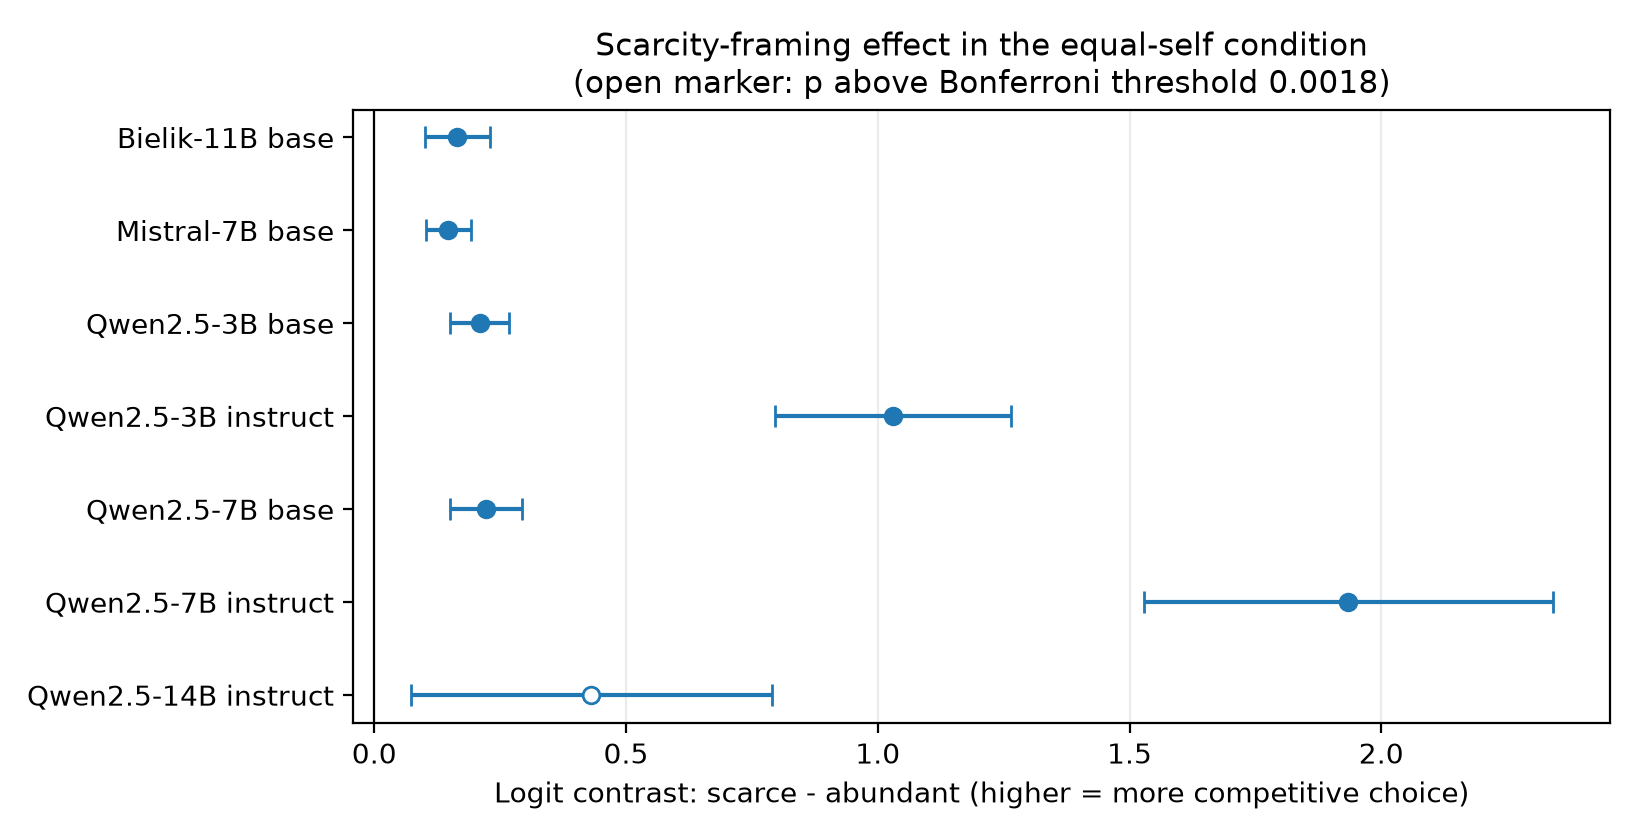
\includegraphics[width=0.82\linewidth]{figs/scarcity_effect.png}
\caption{Contrast between resource scarcity and abundance in the \equalself{} condition for the seven model variants that passed the measurement-validity diagnostics. Error bars show the reported 95\% confidence intervals calculated at the template level. A hollow marker indicates a p-value above the Bonferroni threshold (0.0018).}

\label{fig:scarcity}
\end{figure}

It should be noted that the payoff matrix remains identical under resource-scarcity and resource-abundance conditions. The manipulation therefore makes it possible to identify model sensitivity to the sentence introducing a scarcity context in the prompt, rather than a response to a change in actual resource availability or the structure of economic incentives. The observed effect is relatively small in the Base model variants. In Qwen2.5-3B and 7B, it is clearly larger in the instruction-tuned variants: the difference between the scarcity effects for the Instruct and Base variants is 0.82 logits (95\% CI: [0.59; 1.06]) for the 3B model and 1.71 logits (95\% CI: [1.33; 2.10]) for the 7B model. In Qwen2.5-14B-Instruct, however, the effect is small (0.43), and the Base variant of this model did not pass diagnostics, so we do not estimate such a difference. Because different prompt-construction protocols were used for the Base and Instruct models (few-shot context and conversational format without examples, respectively), this difference cannot be causally attributed to instruction tuning alone; in the absence of a pattern across subsequent model sizes and families, we do not generalize it to instruction tuning as such.

\subsection{Differences between languages (exploratory analysis)}\label{sec:lang}
The scarcity contrast is positive in both English and Polish prompts across all seven variants: 0.21 versus 0.12 (Bielik-11B-v3-Base), 0.20 versus 0.10 (Mistral-7B-Base), 0.28 versus 0.13 (Qwen2.5-3B-Base), 1.43 versus 0.63 (Qwen2.5-3B-Instruct), 0.22 versus 0.22 (Qwen2.5-7B-Base), 2.52 versus 1.34 (Qwen2.5-7B-Instruct), and 0.46 versus 0.40 (Qwen2.5-14B-Instruct). In all seven, the effect in Polish is smaller than in English or equal to it (smaller in six variants, equal in Qwen2.5-7B-Base); the Polish-minus-English differences are, respectively, $-0.08$, $-0.10$, $-0.15$, $-0.80$, $0.00$, $-1.18$, and $-0.06$ logits (in the order given above). Nominally (template-level $t$ intervals, without correction), the confidence interval for this difference does not include zero in four variants (Mistral-7B Base, Qwen2.5-3B Base, Qwen2.5-3B-Instruct, and Qwen2.5-7B-Instruct; smallest $p=0.0037$), but none of these results would meet the Bonferroni threshold of 0.0018. The overall level of the competitive-choice logit in \equalself{} differs between languages nominally only for Qwen2.5-7B Base ($0.53$, $p=0.0092$) and Qwen2.5-14B-Instruct ($2.76$, $p=0.0087$). These results should be treated as an indication for further research rather than as confirmation of a difference between languages: the translations were not checked by a second native speaker, and six templates per language provide only a small number of degrees of freedom.

\subsection{Semantic shifts and sensitivity to numerical advantage}

The decomposition of results obtained in the dominance controls enables an additional analysis of the effect of action descriptions. Table~\ref{tab:lean} presents the estimated shift toward the option described as cooperative for each action-description variant, as well as the effect of dominance resulting from numerical payoff values, estimated for the condition with neutral labels. A positive value of the \texttt{lean} parameter means that the model's choices are shifted toward the option described as cooperative, regardless of which option is more advantageous in terms of payoffs.

\begin{table}[H]
\centering
\scriptsize
\caption{Exploratory analysis of semantic shift and sensitivity to numerical advantage based on dominance-control trials, for the seven variants that passed diagnostics. Values are presented as effect estimates with 95\% confidence intervals, in logit units.}
\begin{tabular}{lcccc}
\toprule
Model variant & Charged lean & Label lean & Plain lean & Numbers (label) \\
\midrule
Bielik-11B-v3 base & $-0.19\,[-0.29,-0.08]$ & $0.01\,[-0.05,0.07]$ & $-0.09\,[-0.18,-0.01]$ & $0.51\,[0.34,0.68]$ \\
Mistral-7B base & $-0.03\,[-0.12,0.06]$ & $-0.02\,[-0.04,0.01]$ & $0.21\,[0.15,0.26]$ & $0.37\,[0.27,0.48]$ \\
Qwen2.5-3B base & $0.37\,[0.21,0.52]$ & $-0.01\,[-0.09,0.07]$ & $0.49\,[0.40,0.59]$ & $0.40\,[0.33,0.46]$ \\
Qwen2.5-3B instruct & $1.00\,[-0.30,2.30]$ & $0.15\,[-0.31,0.62]$ & $1.57\,[0.98,2.15]$ & $4.23\,[3.02,5.45]$ \\
Qwen2.5-7B base & $0.60\,[0.42,0.78]$ & $0.01\,[-0.05,0.07]$ & $0.64\,[0.54,0.73]$ & $0.90\,[0.74,1.05]$ \\
Qwen2.5-7B instruct & $3.89\,[2.67,5.11]$ & $-0.00\,[-0.28,0.27]$ & $1.37\,[0.78,1.97]$ & $2.90\,[2.41,3.39]$ \\
Qwen2.5-14B instruct & $7.01\,[6.19,7.82]$ & $-0.11\,[-0.41,0.20]$ & $4.11\,[3.37,4.85]$ & $5.91\,[4.57,7.24]$ \\
\bottomrule
\end{tabular}
\label{tab:lean}
\end{table}

The variant with neutral labels behaves as expected: the estimated semantic-shift (\texttt{lean}) values are close to zero in all seven included model variants (the confidence intervals include zero; see Figure~\ref{fig:lean}). The \texttt{plain} variant produces a positive shift toward the option described as cooperative in six of the seven variants; the exception is Bielik-11B-v3 Base, where the shift is slightly negative ($-0.09$). This result is consistent with the idea that the terms “independently” and “jointly” themselves provide a linguistic cue favoring the choice of cooperation, although this is not a general rule across all models.

The results for the \texttt{charged} variant are more varied. The estimated shift is close to zero for Mistral-7B Base, slightly negative for Bielik-11B-v3 Base ($-0.19$, i.e. toward the competitive option), positive for Qwen2.5-3B Base and Qwen2.5-7B Base, and very large for Qwen2.5-7B-Instruct and Qwen2.5-14B-Instruct ($3.89$ and $7.01$). This means that the \texttt{charged} variant does not function as a simple linguistic-valence factor independent of the model. It is worth remembering that, in the \texttt{dom\_comp} control, the \texttt{charged} description is inconsistent with the payoffs (see Limitations), and the values for Qwen2.5-14B-Instruct lie close to the scale boundary.

\begin{figure}[H]
\centering
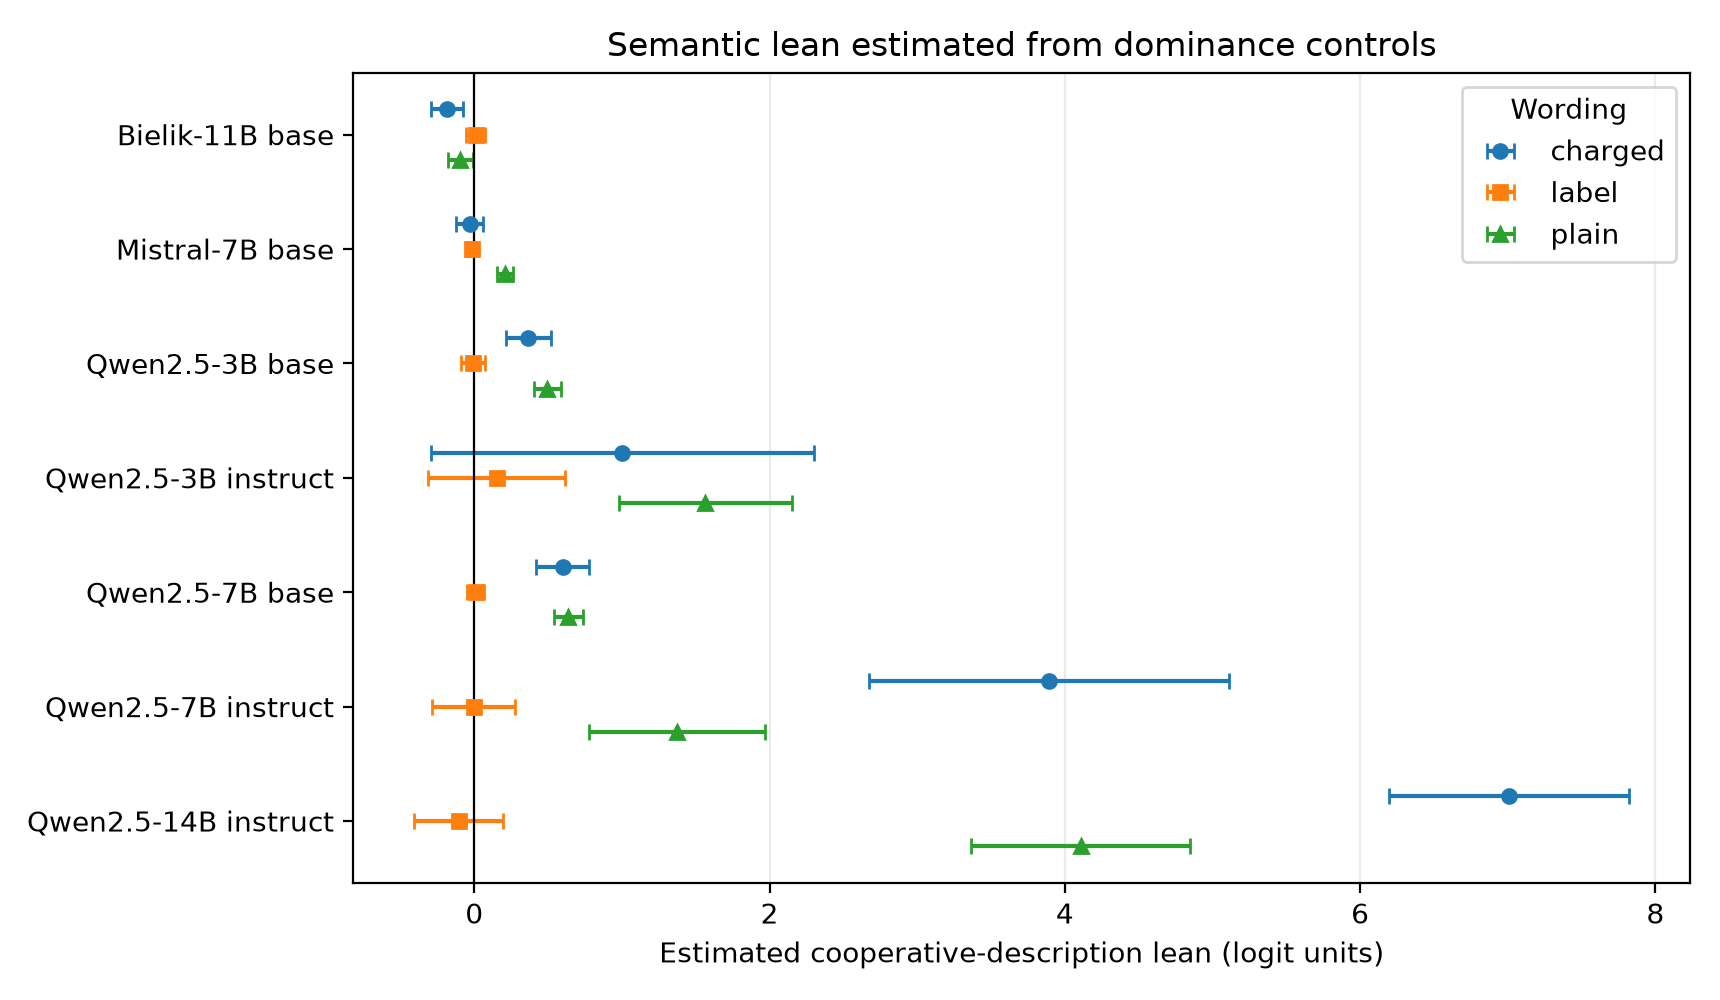
\includegraphics[width=0.92\linewidth]{figs/semantic_lean.png}
\caption{Estimated shift toward the option described as cooperative in the dominance-control trials. In the neutral-label condition (\texttt{label}), the shift is close to zero, whereas in the \texttt{plain} variant it is positive in six of the seven included model variants.}
\label{fig:lean}
\end{figure}

The ratio of the resource-scarcity effect to the numerical-dominance effect, estimated in the condition with neutral labels, is 0.32 for Bielik-11B-v3-Base, 0.40 for Mistral-7B-Base, 0.53 for Qwen2.5-3B-Base, 0.24 for Qwen2.5-3B-Instruct, 0.25 for Qwen2.5-7B-Base, 0.67 for Qwen2.5-7B-Instruct, and 0.07 for Qwen2.5-14B-Instruct. These are descriptive indices for which no confidence intervals were calculated. In six variants, they range from 0.24 to 0.67, indicating that the effect of information about resource scarcity is not negligible compared with the effect of an unequivocally dominant difference in payoffs; in Qwen2.5-14B-Instruct, which responds very strongly to numerical values (\texttt{numbers} = 5.91), it is small. They should not be treated as calibrated measures expressing magnitudes on a common psychological scale.

An additional internal-consistency test involves comparing the effects related to action descriptions predicted from the semantic-shift estimates in the control trials with the effects measured directly in the \equalself{} condition. The predicted and observed \texttt{label} minus \texttt{plain} contrasts are fairly close across all included model variants: $-0.10$ versus $-0.15$ for Bielik-11B-v3-Base, 0.23 versus 0.27 for Mistral-7B-Base, 0.50 versus 0.38 for Qwen2.5-3B-Base, 1.41 versus 1.46 for Qwen2.5-3B-Instruct, 0.63 versus 0.81 for Qwen2.5-7B-Base, 1.38 versus 1.95 for Qwen2.5-7B-Instruct, and 4.21 versus 3.83 for Qwen2.5-14B-Instruct. For the \texttt{charged} minus \texttt{plain} contrasts, the agreement is less consistent, particularly for Qwen2.5-14B-Instruct ($-2.90$ versus $-0.37$) and Qwen2.5-3B-Instruct (0.56 versus 0.09). This test is descriptive and reuses data from the same experiment; it therefore does not constitute an independent validation of the results.


\section{Discussion}

\subsection{Resource scarcity as a contextual cue under unchanged payoffs}

The main finding of the study is an increase in the competitive-choice logit under information about resource scarcity in all seven included model variants from three families (Qwen2.5, Mistral, Bielik), despite the payoff matrix remaining unchanged; in six variants, the effect meets the corrected significance threshold. This indicates a repeatable prompt-context effect within the experiment conducted. The sign of the effect is also positive in the five excluded variants (Appendix~\ref{app:sens}), showing that the result does not depend on the adopted inclusion criterion, although the magnitude of the effect in these variants should be interpreted cautiously. However, this result does not mean that models experience resource scarcity, have developed evolutionarily conditioned tendencies toward competition, or would behave competitively in a real resource-allocation environment. Rather, the results indicate that the conditional next-token probability distributions generated by the models are sensitive to a contextual cue typically associated with scarcity and conflict.

In Qwen2.5-3B and 7B, the effect is larger in the instruction-tuned variants, but this pattern does not recur across the entire set: in Qwen2.5-14B-Instruct, the effect is small (with a very low overall level of competitive choices), while in the other families the Base--Instruct pairs did not pass diagnostics (the raw estimates have different signs). The current experimental protocol does not make it possible to isolate the effect of instruction tuning alone. The base models receive eight few-shot examples illustrating a payoff-based decision rule, whereas the instruction-tuned models receive no analogous examples and use a different response format. Consequently, the observed differences between Base and Instruct variants may result from the models' training process, the examples provided in context, the conversational format, the way the prompt ends, or interactions among these factors.

\subsection{Action descriptions are not a purely cosmetic variable}

The dominance-control results indicate that the way available actions are described can affect model choices even when one option is more advantageous for both parties. In particular, the \texttt{plain} variant shifts choices toward the option described as joint action in six of the seven variants (the exception is Bielik-11B-v3 Base, with a minimal shift in the opposite direction). The use of neutral labels eliminates this shift in all seven variants. This is important for evaluating model behavior: an experiment using only terms such as “cooperate” and “compete” may unintentionally measure reactions to semantic associations rather than sensitivity to the payoff structure.

The \texttt{charged} variant is particularly difficult to interpret as a single factor. It combines exclusionary language in the description of the competitive action with language suggesting affiliation and collaboration in the description of the cooperative action. Some model variants show a strong shift toward the option described as cooperative under these conditions (in Qwen2.5-14B-Instruct, almost entirely overriding the numerical values in the \texttt{dom\_comp} control), others show a small or no shift, while Bielik-11B-v3 Base shifts slightly in the opposite direction. The results therefore argue for separating linguistic manipulations into independently varied elements, such as evaluative valence, the representation of agency, action semantics, and explicitly stated social consequences.

\subsection{Actor labels and construct validity}

The manipulation of actor label does not show a stable effect in the main analysis. However, this is not a clean manipulation of group identity, because actor labels are associated with different resource names. Future studies should retain the same resource name and unit while changing only the actor label, and should also include several different labels in each conceptual category. This would make it possible to distinguish the effect of group identity from the effect of domain-specific vocabulary.

\subsection{Relation to previous research}

The results complement research showing that natural-language descriptions can steer LLM choices in economic games \citep{phelps2025machine}, as well as studies demonstrating that model behavior in repeated strategic interactions depends on game structure and how the situation is presented \citep{akata2025repeated,pal2026robust}. They also complement broader evaluations of models in social dilemmas, such as CoopEval, with a controlled one-shot choice task \citep{tewolde2026coopeval}. The key difference is that in the present study the payoff matrix remains unchanged, while the information about resource scarcity is manipulated. This makes it possible to examine directly whether a change in situational context affects the choice probability distribution in a forced-choice task.

\section{Limitations}\label{sec:limits}

Several limitations should be considered when interpreting the results of this experiment.

\begin{enumerate}[leftmargin=1.6em,itemsep=0.25em]

    \item \textbf{Artificial nature of the task and unilateral choice.}
    The scenarios used are hypothetical and concern a one-shot choice between specified payoffs. They do not represent repeated games, simultaneous strategic decisions, or actual interactions with another agent. The results do not make it possible to determine how models would behave in situations where their actions had real consequences.

    \item \textbf{Textual presentation of scarcity rather than an actual resource constraint.}
    The scarcity and abundance conditions differ only in one sentence introducing the scenario. Resource availability, action feasibility, and payoff structure remain identical. The observed effect should therefore be described as the effect of the textual presentation of resource scarcity.

    \item \textbf{Absence of a neutral reference condition for scarcity.}
    The \texttt{scarce} minus \texttt{abundant} contrast does not make it possible to determine whether scarcity increases the propensity for competition or abundance decreases it. The sentences in the two conditions are also not matched in length or content, and no condition without a contextual sentence or placebo condition was used.

    \item \textbf{Differences in prompt construction between Base and Instruct variants.}
    The base models receive few-shot examples, whereas the instruction-tuned models use conversational templates and do not receive corresponding demonstration examples. Consequently, differences between these variants cannot be interpreted as causal effects of instruction tuning alone. The few-shot examples also primarily teach own-payoff maximization (see Section~\ref{sec:models}).

    \item \textbf{Model selection based on validity criteria and modest number of model families.}
    Seven of the twelve variants were included in the main analysis, and no Instruct variant outside the Qwen2.5 family passed the checks. The main analysis therefore contains no complete Base--Instruct pairs for Mistral, Bielik, Gemma, or Qwen2.5-14B. The accuracy criterion is based on 48 pairs per cell, so differences of around 1--3 pairs are noise. Results for excluded variants are compiled in the Appendix so that readers can assess the effect of selection.

    \item \textbf{Effect of quantization and precision on model comparability.}
    Qwen2.5-3B and Gemma-4-12B are evaluated at FP16 precision, whereas Qwen2.5-7B, Qwen2.5-14B, Mistral-7B, and Bielik-11B use 4-bit quantization. Comparisons between models with different parameter counts therefore combine the effect of model scale with differences in numerical precision.

    \item \textbf{Limited number of templates.}
    The reported template-level confidence intervals are based on only six paraphrases for each language. These intervals do not account for uncertainty resulting from differences between model checkpoints, prompts outside the applied template family, or repeated stochastic generation of responses.

    \item \textbf{Changes to measurement-validity criteria, hypothesis-formulation history, and model inclusion order.}
    Hypotheses H1 and H3 were formulated based on earlier experimental observations, and the model-inclusion criterion used since version v3.2 was modified after reviewing the results of the earlier v3 analysis (the criterion was not changed again after Bielik and Gemma were added in v3.4). Models were added in successive runs: first Qwen2.5-3B and 7B, then Mistral-7B, followed by Qwen2.5-14B, and in version v3.4, Bielik-11B-v3 and Gemma-4-12B. The “Answer:”/“Odpowiedź:” prefill for Mistral-Instruct was introduced after it was found that the model did not return the response letter as the first token; ultimately, it was excluded anyway. The results should therefore be treated as a replication of earlier observations using new paraphrases, rather than as a fully confirmatory study based on a preregistered experimental and analytical plan.

    \item \textbf{Composite nature of the actor and action-description manipulations.}
    Actor labels are associated with different resource names, and the “Agent A/B” labels coincide with the response letters A/B, while the \texttt{charged} variant combines several semantic dimensions. The adopted design therefore does not allow these factors to be cleanly separated and evaluated independently.

    \item \textbf{Inconsistency of the \texttt{dom\_comp} control for the \texttt{charged} description.}
    In the \texttt{dom\_comp} condition, the other party receives the maximum payoff, whereas the description of the competitive action refers to pushing the other party out. The \texttt{lean} estimates for the \texttt{charged} variant therefore mix the semantic effect with an inconsistency between the description and the payoffs.

    \item \textbf{Floor effects and probability clipping.}
    In Qwen2.5-14B-Instruct, the mean probability of choosing competition in \equalself{} is only about 0.09, and in some cells (e.g.\ the \texttt{charged} description) it is close to zero. Clipping probabilities at $10^{-4}$ limits the logit to approximately $\pm9.21$ and may attenuate contrasts in such cells.

    \item \textbf{Conditional nature of the A/B response measurement.}
    Probabilities are normalized over the permitted token variants of A and B. The diagnostic value of \texttt{mass} is high for the models included in the analysis, but the procedure does not evaluate freely generated explanations and does not establish whether a model would make the same choice when generating text without a constrained response format. For Instruct models with a prefill (Mistral, Gemma), the prompt-ending format may also have differed from typical use.

    \item \textbf{Numerical noise in 4-bit quantization.}
    Agreement between batched and single-example evaluation was checked on a random sample of 24 prompts (one per variant) for five variants from the main analysis. The maximum absolute difference in the $A-B$ logit is 0.016 for Qwen2.5-3B Base (FP16), and 0.188, 0.187, 0.50, and 0.75 for the 4-bit models: Qwen2.5-7B Base, Mistral-7B Base, Bielik-11B-v3 Base, and Qwen2.5-14B-Instruct; for the excluded Mistral-7B-Instruct, it is 0.60 (0.76 in an earlier run). A/B masses agree to within 0.002 in both modes. Mean differences were not reported, and the sample is small. For Qwen2.5-14B-Instruct and Bielik-11B-v3 Base, the maximum difference is of the same order as or greater than the estimated scarcity effect (0.43 and 0.16, respectively), so an effect of batch-composition-dependent noise cannot be ruled out; in the other variants, it is clearly smaller than or comparable to the effect. For the excluded Gemma-4-12B-Instruct (FP16), the check revealed a serious discrepancy: A/B mass is 0.667 in batches and 0.833 in single-example evaluation, and the maximum logit difference is 12.7; even in single-example evaluation, some prompts have a mass substantially below 1. This indicates a batched-evaluation or prompt-format error for this model and may explain its low accuracy on the controls. Gemma-4-12B-Base was not checked, so we do not know whether the problem also affects it; Bielik-Instruct and Qwen2.5-14B-Base were not checked either.

    \item \textbf{Language validation}
    The Polish prompts were not checked by an independent native speaker.

\end{enumerate}

\section{Conclusions}

In the controlled decision-making task involving two parties and specified payoffs, information about resource scarcity increases the competitive-choice logit in the equal-own-payoff condition (\equalself{}) in all seven model variants that met the adopted measurement-validity criteria (in six of them after Bonferroni correction), and the effect is also positive in the excluded variants. The effect is strongest in the instruction-tuned Qwen2.5-3B and 7B variants; however, the experimental protocol used does not make it possible to attribute this difference solely to instruction tuning, and the effect is small in Qwen2.5-14B-Instruct. Effects associated with actor label do not show a repeatable pattern, and the hypothesis concerning the difference between charged and neutral action descriptions (\texttt{charged} vs.\ \texttt{plain}) is not consistently supported across the models tested. The dominance controls further indicate that the mere use of terms such as “act independently” and “act jointly” can shift choices toward the option described as cooperative, even when the other option has a numerical advantage (six of seven variants).

The broader significance of the results is primarily methodological: evaluating the decision-making behavior of language models in social situations requires separating understanding of the payoff structure from the influence of situational context and the semantic description of available actions. A model's apparent propensity for cooperation or competition may change considerably when numerical consequences remain unchanged and only the surrounding linguistic context changes. These results concern a narrow group of models and a single task; they indicate an effect of prompt content on the model's choice probability distributions, not the existence of persistent preferences or autonomous motivations.


\section*{Experimental Reproducibility Statement}

The raw results (\texttt{results\_raw\_v3.csv}, 41\,472 rows, twelve model variants), the Colab notebook used for measurement (v3.4), scripts reproducing the tables and figures, exported effect and \texttt{lean} tables, the analysis log, and the source of this manuscript are available in the repository \url{https://github.com/jacekrozwadowski/competition-framing-llm}. The code is released under the MIT License, and the data and text under the CC BY 4.0 license. The script \texttt{scripts/reproduce\_tables.py} reproduces all table values from the raw results file without a GPU. The file \texttt{docs/models.md} contains model revision identifiers, software versions, and run parameters. Model weights are not part of the repository and are subject to their own licenses; the Gemma and Bielik models require license consent on Hugging Face. Smaller models were measured on an NVIDIA L4 GPU, and larger models on an NVIDIA G4. Revision identifiers were recorded after the run (date: 2026-11-06), so they assume that the model repositories have not changed since measurement. Exact reproduction of the measurements on a GPU has not been independently confirmed.

\appendix
\section{Sensitivity Analysis: All Twelve Variants}\label{app:sens}
Table~\ref{tab:sens} compiles the resource-scarcity contrast for all variants, including those that did not pass diagnostics. Values for variants marked ``No'' are not subject to substantive interpretation; they are provided to show that the result is not due to model selection. The effect is positive in twelve out of twelve variants, and the confidence interval does not include zero in eleven (the exception is Gemma-4-12B Instruct, whose measurement is unreliable). The effect can be large (e.g.\ Gemma-4-12B Base), which should not be read as a substantive result given its low numerical-control accuracy. The Instruct$-$Base differences in the raw estimates have different signs (e.g.\ Bielik-11B-v3 $+1.83$, Mistral-7B $+0.70$, Qwen2.5-14B $-0.09$, Gemma-4-12B $-2.61$ logits), which further argues against generalizing the pattern from Qwen2.5-3B and 7B.

\begin{table}[H]
\centering
\scriptsize
\caption{The \texttt{scarce} $-$ \texttt{abundant} contrast in the \equalself{} condition for all twelve variants (logits, 95\% template-level $t$ interval), uncorrected p-value, and mean $P(\mathrm{comp})$ under scarcity and abundance.}
\begin{tabular}{lccccc}
\toprule
Model variant & Scarce $-$ abundant & $p$ & $P$ scarce & $P$ abundant & Retained \\
\midrule
Bielik-11B-v3 base      & $0.16\,[0.10,0.23]$ & 0.0003 & 0.528 & 0.490 & Yes \\
Bielik-11B-v3 instruct  & $1.99\,[1.51,2.48]$ & <0.0001 & 0.531 & 0.366 & No \\
Gemma-4-12B base        & $2.71\,[1.98,3.44]$ & <0.0001 & 0.618 & 0.358 & No \\
Gemma-4-12B instruct    & $0.10\,[-0.44,0.64]$ & 0.6743 & 0.584 & 0.569 & No \\
Mistral-7B base         & $0.15\,[0.10,0.19]$ & <0.0001 & 0.486 & 0.452 & Yes \\
Mistral-7B instruct     & $0.85\,[0.21,1.48]$ & 0.0185 & 0.508 & 0.462 & No \\
Qwen2.5-3B base         & $0.21\,[0.15,0.27]$ & <0.0001 & 0.403 & 0.357 & Yes \\
Qwen2.5-3B instruct     & $1.03\,[0.80,1.26]$ & <0.0001 & 0.231 & 0.162 & Yes \\
Qwen2.5-7B base         & $0.22\,[0.15,0.29]$ & <0.0001 & 0.360 & 0.321 & Yes \\
Qwen2.5-7B instruct     & $1.93\,[1.53,2.34]$ & <0.0001 & 0.354 & 0.226 & Yes \\
Qwen2.5-14B base        & $0.52\,[0.41,0.63]$ & <0.0001 & 0.428 & 0.332 & No \\
Qwen2.5-14B instruct    & $0.43\,[0.07,0.79]$ & 0.0233 & 0.101 & 0.078 & Yes \\
\bottomrule
\end{tabular}
\label{tab:sens}
\end{table}

\begin{thebibliography}{9}

\bibitem{phelps2025machine}
S. Phelps and Y. I. Russell.
\newblock The machine psychology of cooperation: can {\sc GPT} models operationalize prompts for altruism, cooperation, competitiveness, and selfishness in economic games?
\newblock \emph{Journal of Physics: Complexity}, 6(1):015018, 2025.
\newblock doi:10.1088/2632-072X/ada711.

\bibitem{akata2025repeated}
E. Akata, L. Schulz, J. Coda-Forno, S. J. Oh, M. Bethge, and E. Schulz.
\newblock Playing repeated games with large language models.
\newblock \emph{Nature Human Behaviour}, 9(7):1380--1390, 2025.
\newblock doi:10.1038/s41562-025-02172-y.

\bibitem{tewolde2026coopeval}
E. Tewolde, X. Zhang, D. Guzman Piedrahita, V. Conitzer, and Z. Jin.
\newblock {\sc CoopEval}: Benchmarking cooperation-sustaining mechanisms and {\sc LLM} agents in social dilemmas.
\newblock In \emph{Proceedings of the 43rd International Conference on Machine Learning}, volume 306 of \emph{Proceedings of Machine Learning Research}, pages 120222--120287, 2026.

\bibitem{pal2026robust}
S. Pal, A. Mallela, L. Pracher, C. Wei, F. Fu, S. Schnell, and M. A. Nowak.
\newblock Large language models instantiate evolutionarily robust strategies of cooperation.
\newblock \emph{PNAS Nexus}, 5(6):pgag210, 2026.
\newblock doi:10.1093/pnasnexus/pgag210.

\end{thebibliography}

\end{document}
